\documentclass{article}
\usepackage[utf8]{inputenc}
\usepackage[english]{babel}
\usepackage[margin=1in]{geometry}

\usepackage{fancyhdr}
\usepackage{extramarks}
\usepackage{amsmath}
\usepackage{amsthm}
\usepackage{amsfonts}
\usepackage{tikz}
\usepackage[plain]{algorithm}
\usepackage{algpseudocode}
\usepackage{arydshln}
\usepackage{mathtools}
\usepackage{cases}
\usepackage{listings}
\usepackage[numbered]{mcode}
\usepackage{booktabs}
\usepackage{graphicx}
\usepackage{subfigure}

\usepackage{blindtext}
\usepackage{amssymb}
\usepackage{hyperref}
\hypersetup{
    colorlinks=true,
    linkcolor=blue,
    filecolor=magenta,
    urlcolor=cyan,
}
\lstset{basicstyle=\ttfamily,
    showstringspaces=false,
    commentstyle=\color{red},
    keywordstyle=\color{blue}
}

\urlstyle{same}

%\newtheorem{theorem}{Theorem}
\newtheorem{theorem}{Theorem}[section]
\newtheorem{corollary}{Corollary}[theorem]
\newtheorem{lemma}[theorem]{Lemma}
\theoremstyle{remark}
\newtheorem*{remark}{Remark}

\theoremstyle{definition}
\newtheorem{definition}{Definition}[section]

\title{CS 250 - Computer Architecture \\ Homework 1 Written}
\author{Jincheng He Email: jincheng.he@dukekunshan.edu.cn}
%\date{October 2019}

\begin{document}

    \maketitle


    \section{Question 1 Representing Datatypes in Binary}
    \begin{enumerate}
        \item[(a)] Convert $+47_{10}$ to 8-bit 2s complement integer representation in binary and hexadecimal.

        \begin{table}[!htbp]
            \centering
            \label{tab:q1_a}
            \begin{tabular}{cc}
                \toprule
                & remainder \\
                \midrule
                $47\div 2 = 23$ & 1         \\
                $23\div 2 = 11$ & 1         \\
                $11\div 2 = 5$  & 1         \\
                $5\div 2 = 2$   & 1         \\
                $2\div 2 = 1$   & 0         \\
                $1\div 2 = 0$   & 1         \\
                \bottomrule
            \end{tabular}
            \caption{Process of Calculating}
        \end{table}

        The computing process is as table~\ref{tab:q1_a}. So the 8-bit 2s complement integer representation in binary is $\left( 00101111 \right)_2$. So natually the hexadecimal is 0x2F.
        \item[(b)] Convert $-13_{10}$ to 8-bit 2s complement integer representation in binary and hexadecimal.

        First we need to find out the 2s complement integer representation for $+13_{10}$. Similarly, the process is in table~\ref{tab:q1_b}.
        \begin{table}[!htbp]
            \centering
            \label{tab:q1_b}
            \begin{tabular}{cc}
                \toprule
                & remainder \\
                \midrule
                $13\div 2 = 6$ & 1         \\
                $6\div 2 = 3$  & 0         \\
                $3\div 2 = 1$  & 1         \\
                $1\div 2 = 0$  & 1         \\
                \bottomrule
            \end{tabular}
            \caption{Process of Calculating}
        \end{table}

        So the 8-bit 2s complement integer representation in binary for $+13_{10}$ is $\left( 00001101 \right)_2$. Then for $-13_{10}$, we just need to flip each bit, and then add one, which is $\left( 11110011 \right)_2$. And then natually, the hexadecimal for $-13_{10}$ is 0xF3.
        \item[(c)] Convert $+47.0_{10}$ to 32-bit IEEE floating point representation in binary and hexadecimal.

        First, the binary for $+47.0_{10}$ is $\left( 00101111 \right)_2$. So it is also equal to $1.01111\times 2^5$.

        Sign: it is positive, so it is 0.

        Exponent: $127+5=132$, which is $\left( 1000 0100 \right)_2$.

        Mantissa: 1.011 1100 0000 0000 0000 0000.

        So the 32-bit IEEE floating point representation is: 0 1000 0100 011 1100 0000 0000 0000 0000.

        So natually, the hexadecimal is: 0x423C0000.

        \item[(d)] Convert $-0.375_{10}$ to 32-bit IEEE floating point representation in binary and hexadecimal.

        First, $0.375_{10} = 0 + \frac{1}{4} + \frac{1}{8}$. So the binary is $0.011$, which is also equal to $1.1 \times 2^{-2}$.

        Sign: it is negative, so it is 1.

        Exponent: $127 - 2 = 125$, which is $\left( 0111 1101 \right)$.

        Mantissa: 1.100 0000 0000 0000 0000 0000.

        So the 32-bit IEEE floating point representation is: 1 0111 1101 100 0000 0000 0000 0000 0000.

        So natually, the hexadecimal representation is: 0xBEC00000.
        \item[(e)] Represent the ASCII string "String for 250!" (not including the quotes) in hexadecimal.

        According to the ASCII table, the answer should be: 0x 53 74 72 69 6E 67 20 66 6F 72 20 32 35 30 21.
        \item[(f)] Give an example of a number that cannot be represented as a 32-bit signed integer.

        The range for 32-bit integer is $-2^{31}$ to $2^{31} - 1$. So the integer which is not in this range cannot be representd as a 32-bit signed integer, such as $2^{31}$ cannot be represented.


    \end{enumerate}


    \section{Question 2 Memory as an Array of Bytes}
    \begin{enumerate}
        \item[a. ]
        Where do each of the following variables live (global data, stack, or heap)?
        \begin{enumerate}
            \item[a. ] a

            Stack.
            \item[b. ] b\_ptr

            Stack.
            \item[c. ] *b\_ptr

            Heap.
            \item[d. ] e\_ptr

            Global data.
            \item[e. ] *e\_ptr

            Global data.
        \end{enumerate}
        \item[b. ] What is the value returned by main()?

        It should return 0.
    \end{enumerate}


    \section{Question 3 Compiling and Testing C Code}
    When I type
    \begin{lstlisting}[language=bash]
        g++ -O0 -o myProgramUnopt prog.c
    \end{lstlisting}
    the user running time on my machine is 0.54s.

    When I type
    \begin{lstlisting}[language=bash]
        g++ -O3 -o myProgramOpt prog.c
    \end{lstlisting}
    the user running time on my machine is 0.27s.

    The screenshot is as figure~\ref{fig:optUnoptCompare}.
    \begin{figure}[!htbp]
        \centering
        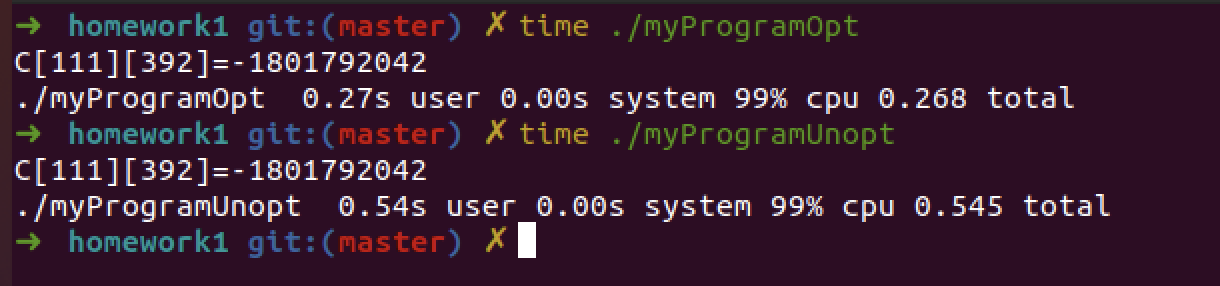
\includegraphics[width=0.8\textwidth]{img/optUnoptCompare.png}
        \caption{Screenshot of the comparison}
        \label{fig:optUnoptCompare}
    \end{figure}


    \section{One Point Extra Credit}
    The fish picture for one point extra credit is as figure~\ref{fig:fish}.
    \begin{figure}[!htbp]
        \centering
        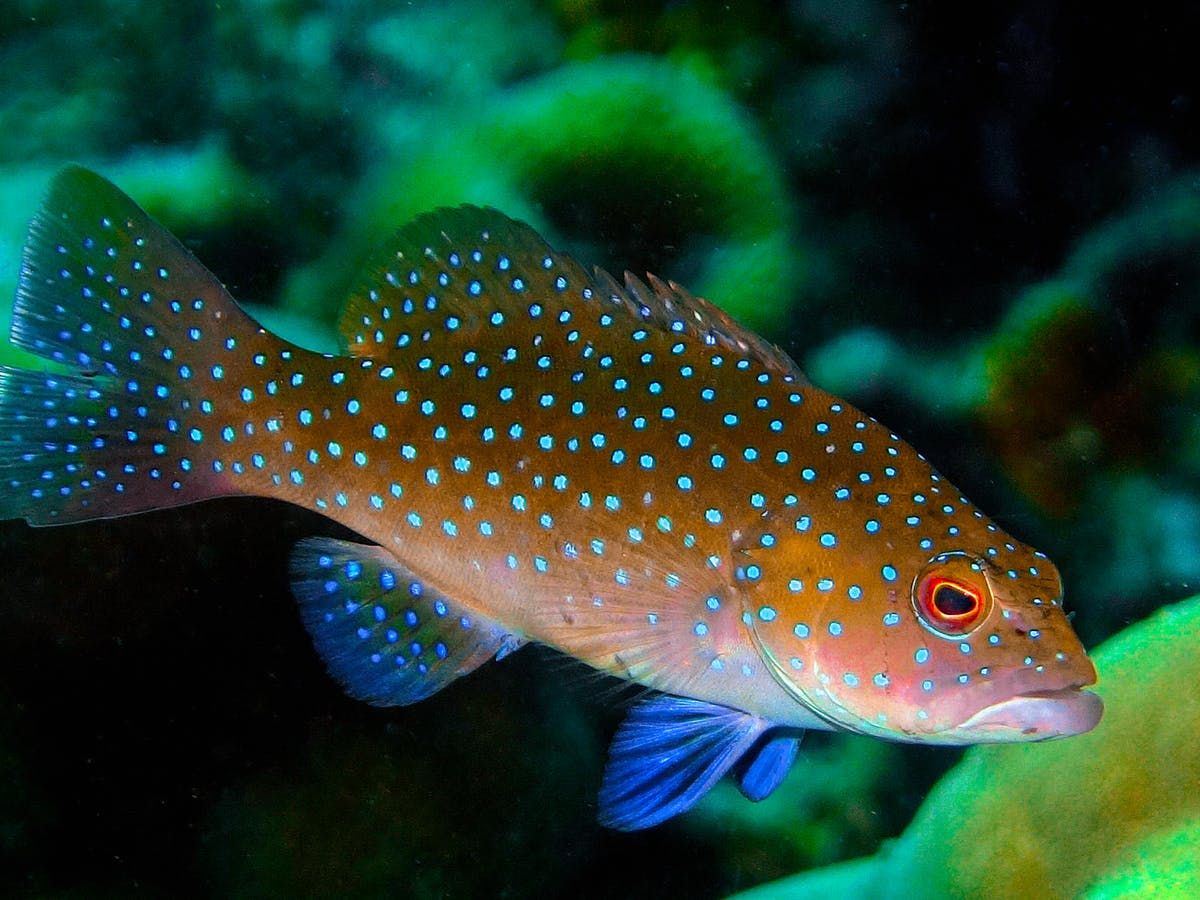
\includegraphics[width=0.4\textwidth]{img/fish.jpg}
        \caption{Fish picture for one point extra credit}
        \label{fig:fish}
    \end{figure}

\end{document}